% !TEX encoding = UTF-8
% !TEX TS-program = pdflatex
% !TEX root = ../tesi.tex
% !TEX spellcheck = it-IT

%**************************************************************
\chapter{Descrizione dello stage}
\label{cap:descrizione-stage}
%**************************************************************

\intro{Questo capitolo tratta dettagliatamente delle attività di pianificazione, studio, analisi, progettazione e sviluppo, svolte durante lo stage.}

%**************************************************************
\section{Pianificazione}
Le attività sono state pianificate prima dell'inizio dello stage. Per conseguire gli obiettivi sono state previste circa 300 ore, suddivise in 40 ore settimanali per 8 settimane. Lo stage è iniziato il giorno 01/10/2015 ed è terminato il 27/11/2015. La pianificazione ha subito una leggera modifica nelle attività, in quanto ho privilegiato lo sviluppo del nuovo modulo \textit{Bdrim} anziché il \textit{porting} del progetto \textit{Dre}. Ogni periodo è stato suddiviso in varie attività. Tali attività sono state suddivise in ulteriori sotto-attività. Di queste sotto-attività viene riportato il diagramma di \gls{gantt}.
\begin{itemize}
	\item \textbf{Prima settimana:}
	\begin{itemize}
		\item Studio del \gls{framework} Play;
		\item Studio del linguaggio di programmazione Scala;
		\item Studio del \textit{database} OrientDB;
		\item Studio del progetto preesistente.
	\end{itemize}
	\item \textbf{Seconda e terza settimana: }migrazione dalla tecnologia MongoDB a OrientDB e \textit{porting} all'ultima versione di Play;
	\item \textbf{Quarta settimana:} Analisi dei requisiti del nuovo modulo;
	\item \textbf{Quinta settimana:} Progettazione architetturale;
	\item \textbf{Sesta e settima settimana:} Implementazione modulo esterno;
	\item \textbf{Ottava settimana:} Test.
\end{itemize}

La figura \ref{fig:ScreenShot2016-01-06at17} rappresenta il diagramma di \textit{Gantt} utilizzato per la pianificazione delle attività.
\begin{figure}[h]
\centering
\includegraphics[width=1.2\linewidth, height=0.45\textheight]{"immagini/piano-di-lavoro"}
\caption[Diagramma di Gantt dello stage]{Diagramma di Gantt dello stage}
\label{fig:ScreenShot2016-01-06at17}
\end{figure}


%**************************************************************
\newpage
\section{Studio del dominio}
Per evitare di incorrere in gravi ritardi e considerata la particolare tecnologia utilizzata, ho studiato e approfondito la mia conoscenza delle tecnologie, attingendo a una documentazione adeguata. Durante la redazione del \textit{Piano di Lavoro}, tenendo conto della propria inesperienza con le tecnologie richieste ho deciso di prevedere un periodo di \gls{slack} per ogni attività con alta criticità, in modo che un eventuale ritardo non andasse ad influenzare la durata totale del progetto.


\subsection*{Scala}
Prima dell'inizio dello stage non avevo conoscenze del linguaggio di programmazione Scala. Per apprendere il linguaggio ho seguito il corso di \textit{Functional Programming Principles in Scala}\footnote{\url{https://www.coursera.org/course/progfun}} e i tutorial presenti nel sito ufficiale\footnote{\url{http://www.scala-lang.org/}}. Entrare nel meccanismo della programmazione funzionale non è stato facile, ma il vasto numero di esempi ed esercizi mi hanno aiutato a capire il concetto che sta alla base di tale programmazione.

\subsection*{Play Framework}
Successivamente ho cominciato lo studio del \gls{framework} che avrei utilizzato durante la realizzazione del progetto. Grazie a un'ottima documentazione\footnote{\url{https://www.playframework.com/documentation/2.4.x/Home}} e ai \textit{tutorials} presenti nel sito di Play\footnote{\url{https://www.playframework.com/documentation/2.4.x/Tutorials}}, l'apprendimento dei concetti principali è stato facile.

\subsection*{OrientDB}
Per lo studio del \textit{database} OrientDB ho seguito il corso online offerto da \textit{Udemy}\footnote{\url{https://www.udemy.com/orientdb-getting-started/}}. Il corso fornisce una panoramica completa sui modelli supportati da OrientDB, con una maggiore considerazione sul modello a grafo.

\section{Analisi dei requisiti}
L'applicativo viene utilizzato come modulo dalla piattaforma di raccolta dati \textit{Bdrim}. \textit{Bdrim} è stato realizzato in un precedente progetto di stage con la collaborazione di Alos S.r.l..\\
L'applicativo \textit{Tres} è stato progettato per una tipologia di utente:
\begin{itemize}
	\item La piattaforma \textit{Bdrim}, che usufruisce delle \gls{api} fornite da \textit{Tres}.
\end{itemize}
Durante l'attività di analisi ho fatto molteplici riunioni di tipo \textit{brainstorming} da cui sono emersi la maggior parte dei requisiti. Tali requisiti sono stati raccolti, in forma tabellare, in un documento di testo, in modo da poter essere sempre disponibile per la consultazione e la modifica. Essi sono stati divisi per tipo, utilizzando da seguente notazione:\\
R[importanza][tipologia][codice]
\begin{itemize}
	\item \textit{Importanza} può assumere i seguenti valori:
	\begin{itemize}
		\item \textbf{OBB:} requisito obbligatorio. Il soddisfacimento è necessario per il raggiungimento degli obiettivi dello \textit{stage};
		\item \textbf{DES:} requisito desiderabile. L'implementazione non è fondamentale, ma dà valore aggiunto al prodotto.
	\end{itemize}
	\item \textit{Tipologia} può assumere i seguenti valori:
	\begin{itemize}
		\item \textbf{F}: requisiti funzionali. Specifica una funzionalità che il software deve avere;
		\item \textbf{V}: requisiti di vincolo. Specifica il vincolo che il software deve avere;
		\item \textbf{P}: requisiti di prestazione. Specifica un vincolo di performance che il software deve fornire. 
	\end{itemize}
\end{itemize}
\newpage
Riporto di seguito la tabella con i requisiti individuati e una breve descrizione per ognuno di essi:
\begin{table}[h]
	\begin{tabular}{|p{0.2\textwidth}|p{0.7\textwidth}|}
		\midrule
		R[OBB][F]1 & Il sistema deve permettere l'inserimento di un nuovo comportamento \\ \midrule
		R[OBB][F]2 & Il sistema deve restituire un messaggio di segnalazione in caso di errore durante il salvataggio \\ \midrule
		R[OBB][F]3 & I dati ricevuti devono essere in formato \gls{JSON} \\ \midrule
		R[OBB][F]4 & I dati inviati devono essere in formato \gls{JSON} \\ \midrule
		R[OBB][F]5 & Il sistema deve restituire un messaggio di errore in caso di \gls{JSON} non valido \\ \midrule
		R[OBB][F]6 & Devono essere inseriti almeno 100 comportamenti per produrre la raccomandazione \\ \midrule
		R[OBB][F]7 & Il sistema deve restituire un messaggio di conferma quando l'algoritmo è pronto a produrre una raccomandazione \\ \midrule
		R[OBB][F]8 & Il sistema deve permettere il calcolo dell'entropia del \textit{dataset} \\ \midrule
		R[OBB][F]9 & Il sistema deve permettere il calcolo del guadagno di informazione del \textit{dataset} \\ \midrule
		R[OBB][V]10 & Il sistema deve permettere la costruzione ricorsivamente dell'albero di decisione \\ \midrule
		R[OBB][V]11 & Il sistema deve permettere la creazione di tanti nodi quanti sono i possibili valori dell'attributo scelto \\ \midrule
		R[OBB][V]12 & L'algoritmo di costruzione dell'albero deve fermarsi quando tutte le istanze di un nodo appartengono alla stessa classe \\ \midrule	
		R[OBB][F]13 & Il sistema deve permettere di ricevere una richiesta per classificare un comportamento vuoto \\ \midrule
		R[OBB][F]14 & Il sistema, per la richiesta con un comportamento vuoto, deve restituire tutte le raccomandazioni con le percentuale calcolate in base al \textit{dataset} \\ \midrule
		R[OBB][F]15 & Il sistema deve permettere di classificare un comportamento dell'utente \\ \midrule
		\bottomrule
		
	\end{tabular}
\end{table}
		
\newpage
\begin{table}[h]
	\begin{tabular}{|p{0.2\textwidth}|p{0.7\textwidth}|}
		\midrule
		R[OBB][F]16 & Il sistema deve fornire una raccomandazione o più in base alla classificazione del comportamento \\ \midrule
		R[OBB][F]17 & Il sistema deve fornire insieme alla raccomandazione la percentuale di adeguatezza \\ \midrule
		R[OBB][V]18 & Il sistema deve permettere la modifica dell'albero di decisione ogni 24 ore \\ \midrule
		R[OBB][V]19 & Devono essere rispettate le metriche sulla stesura del codice riportate nella sezione \ref{metriche} \\ \midrule
		R[DES][F]20 & Devono essere implementati nuovi algoritmi basati sulla teoria de giochi \\ \midrule
		R[DES][V]21 & Devono essere implementati nuovi algoritmi di \textit{clustering} \\ \midrule
		R[DES][V]22 & Deve essere sviluppato il pannello di amministrazione \\ \midrule
		R[OBB][P]23 & Il database deve essere in grado di memorizzare almeno 100.000 record al secondo \\ 
		
		\bottomrule
		
	\end{tabular}
	\caption{Tabella dei requisiti}
\end{table}

\section{Progettazione architetturale}
Questa sezione ha lo scopo di descrivere l'architettura generale e i \textit{design pattern} utilizzati durante la realizzazione del progetto.
\subsection{Architettura generale}
Come ho già anticipato il modulo \textit{Tres} deve essere utilizzabile dalla piattaforma \textit{Bdrim}.  I moduli hanno lo scopo di aumentare l'indipendenza tra le sue parti costituenti e facilitare la manutenzione. Infatti, questi sistemi durante la loro vita subiscono numerose modifiche: per eliminare difetti, per potenziare delle funzionalità o addirittura superare quelle obsolete ed implementarne di nuove. La coppia \textit{Tres-Bdrim} può essere vista come il binomio di due componenti indipendenti tra di loro che comunicano utilizzando lo stile \gls{REST}. Ho deciso di utilizzare il formato \gls{JSON} come formato di rappresentazione dei dati, poiché si integra perfettamente con il \gls{framework} utilizzato e il linguaggio Scala.\\
Entrambe le componenti sono basate su un'architettura di tipo \gls{mvc}. Nella seguente figura è possibile avere una visione d'insieme del progetto.

\begin{figure}[h]
\centering
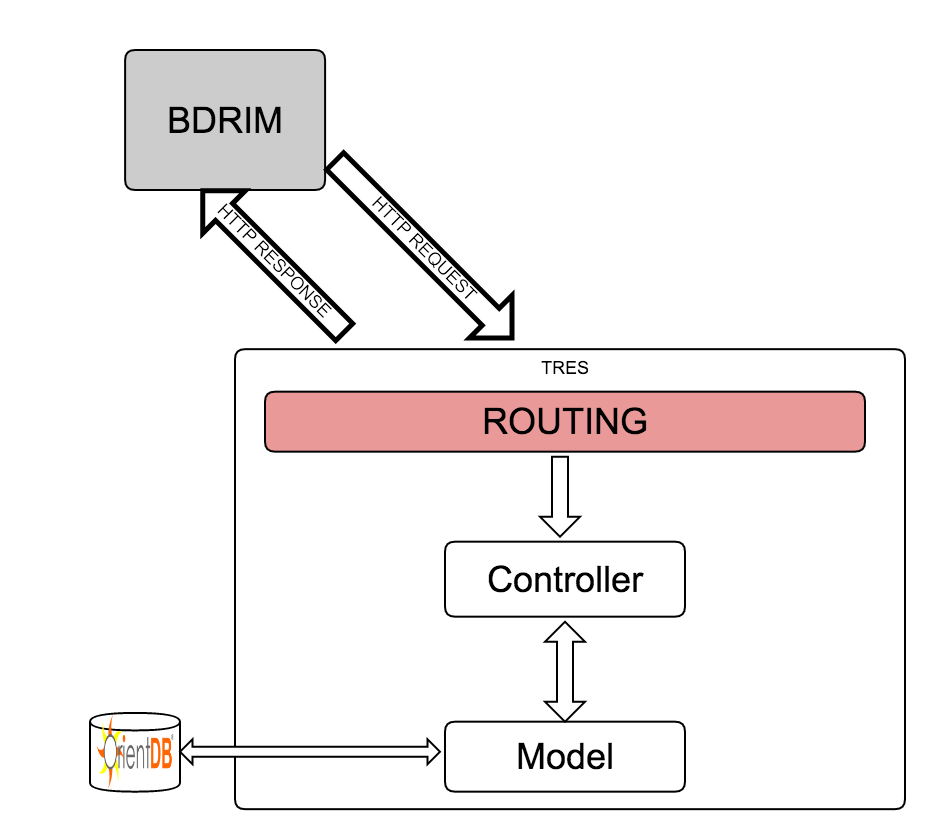
\includegraphics[width=1\linewidth]{immagini/generalGliffy}
\caption[Visione d'insieme dei due componenti]{Visione d'insieme dei due componenti}
\label{fig:generalGliffy}
\end{figure}

\newpage
Dal service \textit{Bdrim} arriva una richiesta \textit{Http} che viene instradata a una classe di un \textit{controller}  mediante il file \textit{routes}. Il \textit{controller} termina la sua esecuzione restituendo un oggetto \gls{JSON} che contiene:
\begin{itemize}
	\item i parametri corretti se la richiesta è andata a buon fine;
	\item un messaggio di successo, nel caso il metodo non preveda il ritorno di alcun parametro (es. salvataggio sul \textit{database});
	\item un messaggio di errore, nel caso la richiesta non vada a buon fine.
\end{itemize}

\subsection{Archittetura dell'applicativo}
L'architettura che ho realizzato segue il \textit{design pattern} \gls{mvc}. I tre \textit{package} creati sono \textit{models, views, controllers}. Il \textit{package views} al momento non viene utilizzato, potendo essere esteso in un progetto futuro, creando un interfaccia di amministrazione o visualizzazione dei dati oppure implementando nuove funzionalità. Sarà ora presentata una visione ad alto livello, le cui componenti verranno analizzate in seguito più dettagliatamente.

\begin{figure}[h]
\centering
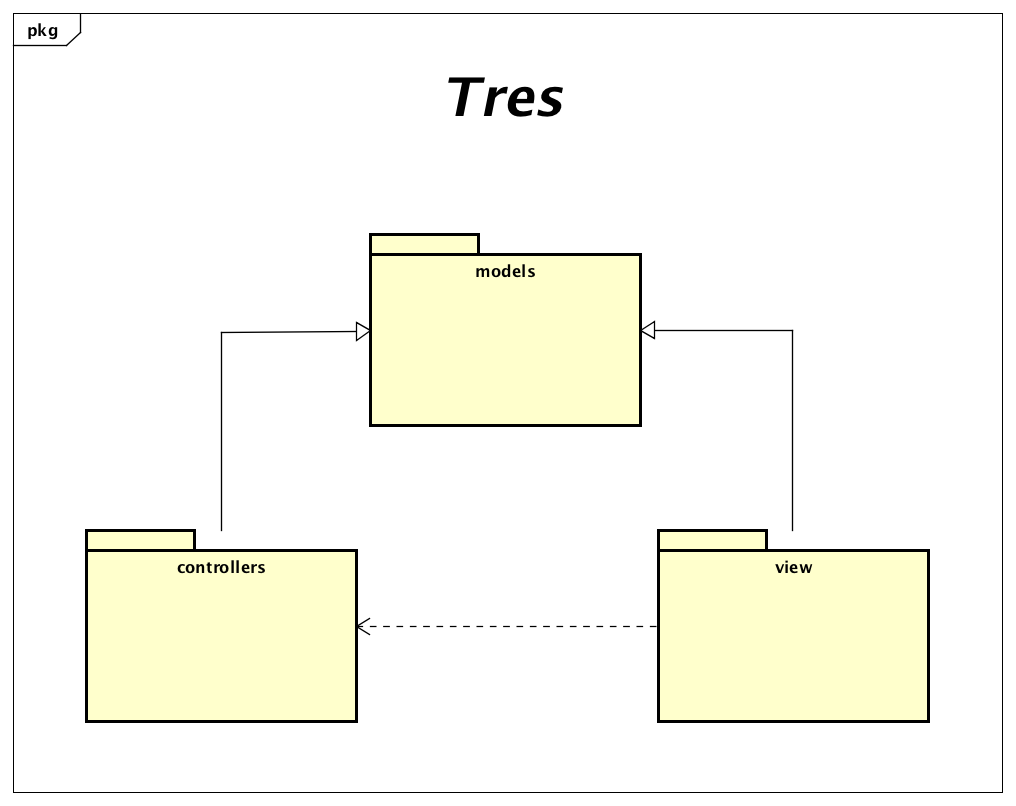
\includegraphics[width=0.9\linewidth]{immagini/tres}
\caption[Visione ad alto livello dell'architettura realizzata]{Visione ad alto livello dell'architettura realizzata}
\label{fig:arcGenerale}
\end{figure}

\subsection*{models}
Il \textit{package} \textit{models} contiene la logica di \textit{business} ed è la componente \gls{mvc} dedicata all'accesso ai dati. Il \textit{package} non fornisce direttamente l'accesso ai dati, ma si preoccupa di creare il necessario livello di astrazione tra il formato in cui i dati sono memorizzati alla fonte e il formato in cui i livelli di \textit{controllers e views} si aspettano di riceverli.

\begin{figure}[h]
\centering
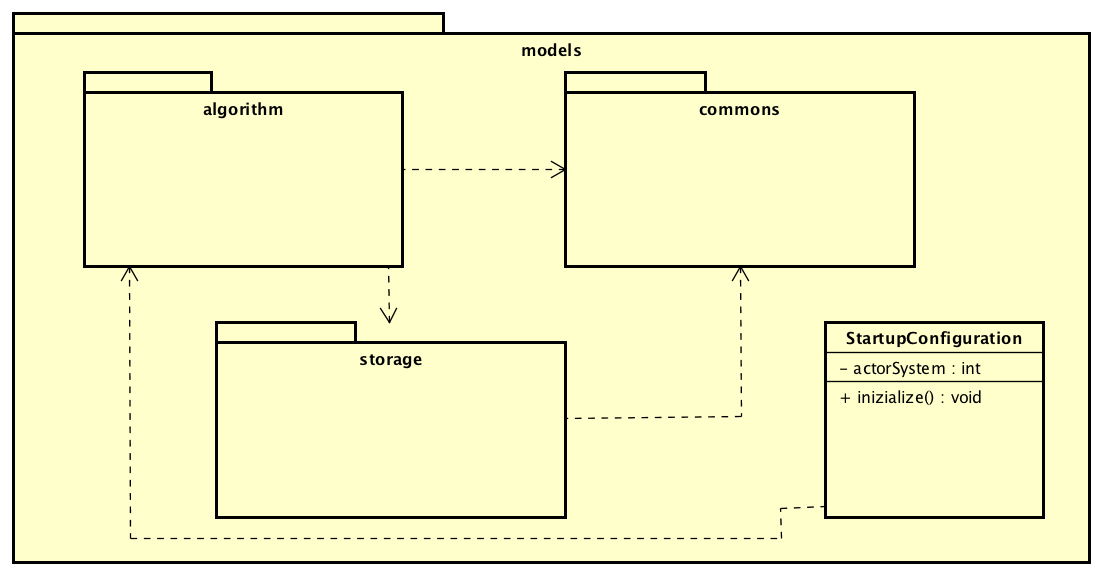
\includegraphics[width=0.9\linewidth]{immagini/tres-models}
\caption[Diagramma del package models]{Diagramma del package models}
\label{fig:tres-models}
\end{figure}

\newpage
Il core dell'applicazione viene implementato dal \textit{package models}, che incapsulando lo stato dell'applicazione definisce i dati e le operazioni che possono essere eseguite su questi.

\subsubsection*{Classi contenute}
\begin{itemize}
	\item \textbf{StartupConfiguration:} contiene la configurazione che fa partire, ogni 24 ore, l'algoritmo dedicato alla creazione dell'albero decisionale su cui si basano tutte le raccomandazioni.
\end{itemize}

\subsubsection*{Package contenuti}
	
	\subsubsection*{algorithm}
	\begin{figure}[h]
	\centering
	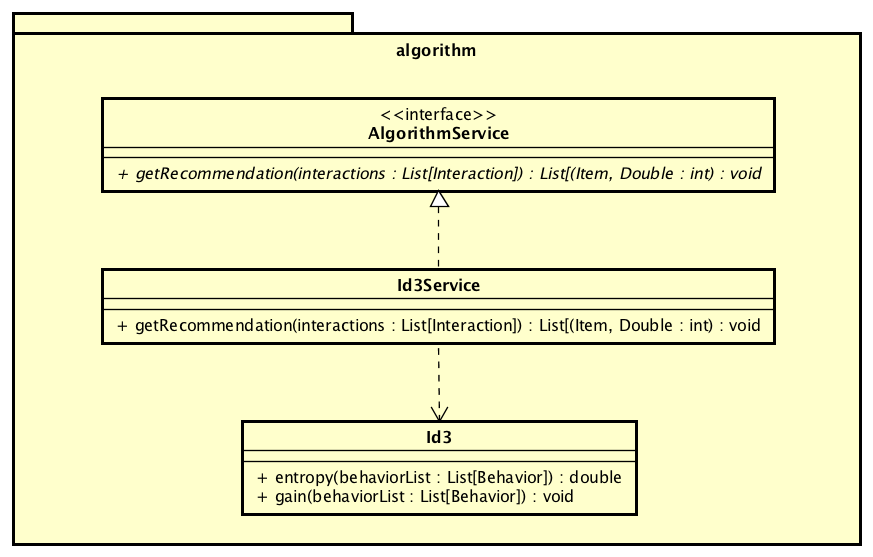
\includegraphics[width=0.8\linewidth]{immagini/tres-algorithm}
	\caption[Diagramma del package algorithm]{Diagramma del package algorithm}
	\label{fig:tres-algorithm}
	\end{figure}
	Il \textit{package} contiene tutta la logica per costruire alberi di decisione e offrire le raccomandazioni con le rispettive probabilità. Infatti, ad ogni raccomandazione o insieme di raccomandazioni viene fornita anche le percentuale di scelta che ha il prodotto. Utilizza il \textit{package storage} per aggiornare i dati presenti nel \textit{database};
	
	\subsubsection*{commons}
	\begin{figure}[h]
	\centering
	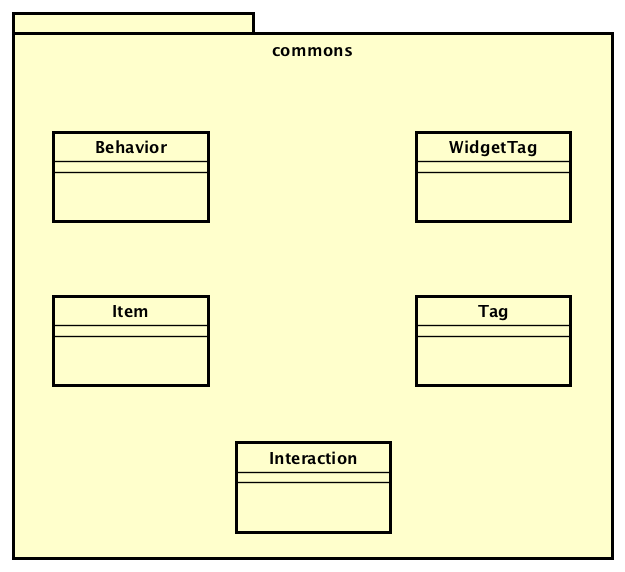
\includegraphics[width=0.6\linewidth]{immagini/tres-commons}
	\caption[Diagramma del package commons]{Diagramma del package commons}
	\label{fig:tres-commons}
	\end{figure}
	Il \textit{package} contiene la struttura delle classi di tutti i componenti dell'applicazione. Include anche le funzioni per passare da oggetti del \textit{model} ad oggetti \gls{JSON} e viceversa.
	
\subsubsection*{storage}
	\begin{figure}[h]
	\centering
	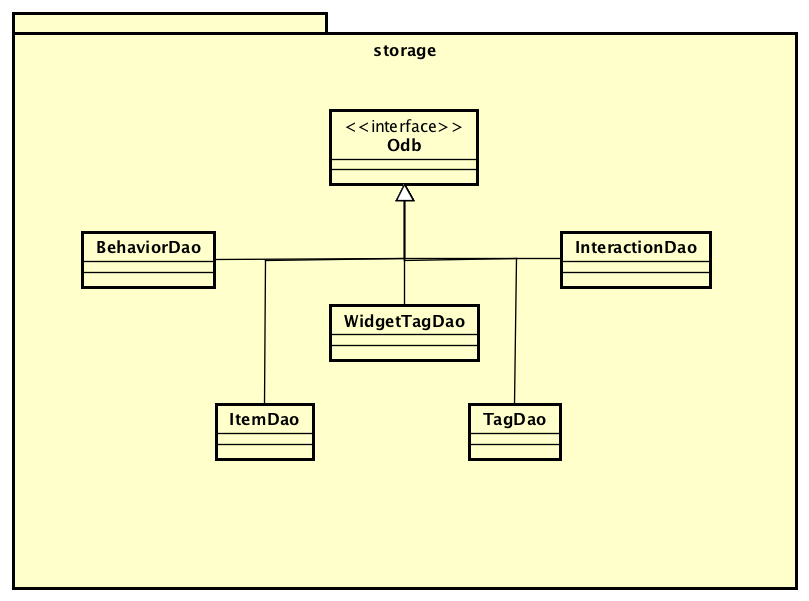
\includegraphics[width=0.55\linewidth]{immagini/tres-storage}
	\caption[Diagramma del package storage]{Diagramma del package storage}
	\label{fig:tres-storage}
	Il \textit{package} contiene la logica di accesso ai dati. Le classi all'interno si occupano di interagire con il \textit{database.} 
\end{figure}

\newpage
\subsection*{controllers}
Il \textit{package} contiene le componenti che gestiscono la parte \textit{controller} dell'applicazione. La classe \textit{BridgeController} contiene i metodi necessari da invocare come risposta alla chiamata di una determinata richiesta. Vi è un'interazione con il \textit{package models} poiché in esso vengono depositati e prelevati i dati necessari alla richieste. Inoltre ha una dipendenza uscente verso il \textit{package views}.
\begin{figure}[h]
\centering
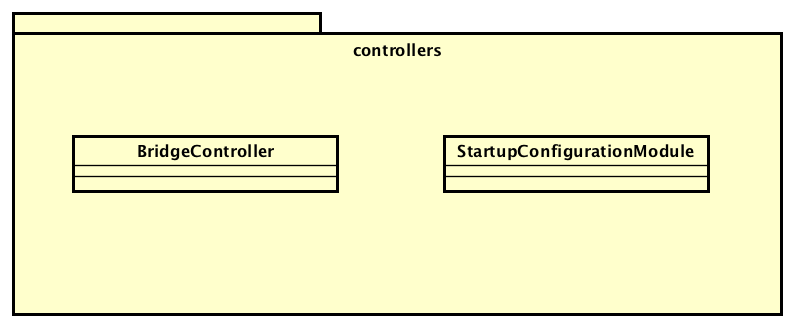
\includegraphics[width=0.7\linewidth]{immagini/tres-controller}
\caption[Diagramma del package controllers]{Diagramma del package controllers}
\label{fig:tres-controller}
\end{figure}

\subsection{Modello del database}
Nella rappresentazione grafica del \textit{database}, il grafo viene rappresentato mediante
un disegno in cui ai nodi si fanno corrispondere piccoli cerchi e agli spigoli frecce che rappresentano la relazione tra due vertici. La direzione degli spigoli è importante perché dà un senso alla relazione.\\
Per interfacciarmi con il \textit{database} ho usato le \gls{api} \textit{Blueprints}\footnote{\url{https://github.com/tinkerpop/blueprints}} sviluppate dal \gls{framework} \textit{Tinkerpop}\footnote{\url{http://tinkerpop.incubator.apache.org/}}. In particolare, \textit{Tinkerpop} è un set di interfacce e specifiche per lavorare con grafi, che OrientDB supporta dalla versione 0.9.22.
\begin{figure}[h]
\centering
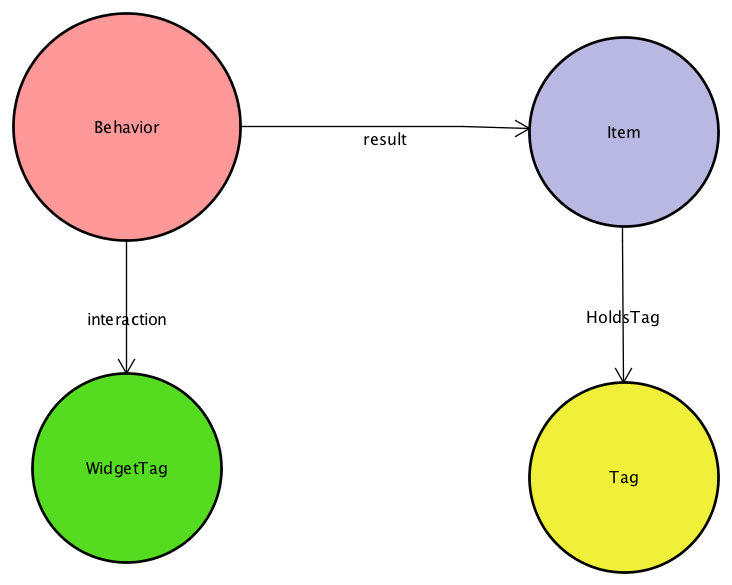
\includegraphics[width=0.6\linewidth]{immagini/db-a-graffo}
\caption[Modello a grafo del database]{Modello a grafo del database}
\label{fig:db-a-graffo}
\end{figure}

\subsection{Design pattern utilizzati}
Di seguito sono elencati i \textit{design pattern} utilizzati durante lo sviluppo con i rispettivi diagrammi di esempio .
\begin{itemize}
	\item \gls{mvc}
	\begin{figure}[h]
\centering
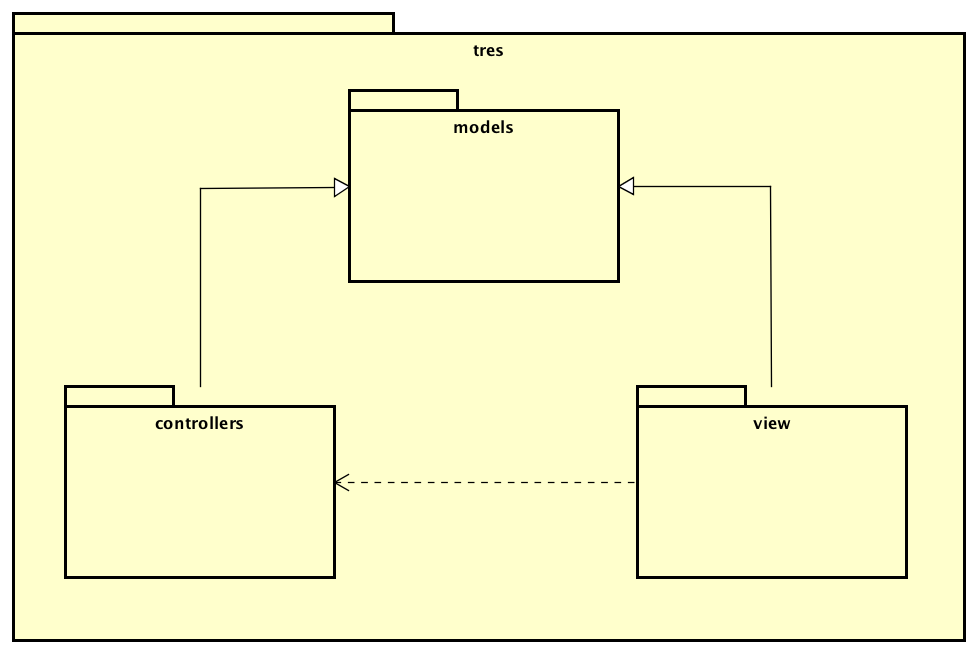
\includegraphics[width=0.5\linewidth]{immagini/esempioMVC}
\caption[Utilizzo del design pattern MVC]{Contesto d'utilizzo del design pattern MVC}
\label{fig:esempioMVC}
\end{figure}

	\begin{itemize}
		\item \textbf{Descrizione:} prevede la separazione in tre componenti:
		\begin{itemize}
			\item \textit{model}: fornisce i metodi per accedere ai dati utili dell'applicazione;
			\item \textit{view}: visualizza i dati contenuti nel model e si occupa delle interazioni esterne;
			\item \textit{controller:} esegue funzionalità e modifica lo stato del \textit{model} e/o \textit{view}.
		\end{itemize}
		\item \textbf{Contesto d'utilizzo:} il \textit{pattern} viene implementato dal \gls{framework} utilizzato e permette di organizzare modularmente gli strati software.
	\end{itemize}
	\item \gls{dao}
	\begin{figure}[h]
\centering
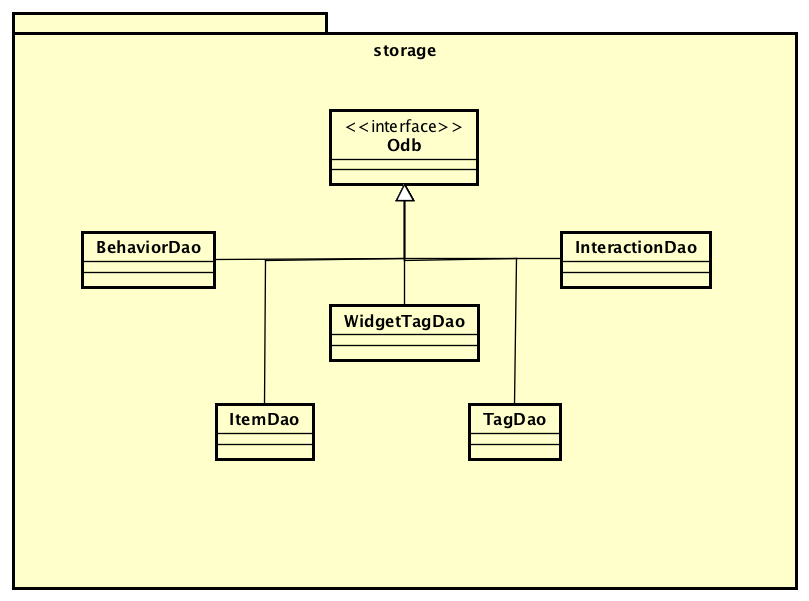
\includegraphics[width=0.5\linewidth]{immagini/tres-storage}
\caption[Utilizzo del design pattern DAO]{Contesto d'utilizzo del design pattern DAO}
\label{fig:tres-storage}
\end{figure}

	\begin{itemize}
		\item \textbf{Descrizione:} \textit{pattern} architetturale utilizzato per la gestione della persistenza. Mantiene una rigida separazione tra le componenti dell'applicazione, in questo caso tra \textit{model e controller}.
		\item \textbf{Contesto d'utilizzo:} viene implementato nel \textit{package storage} per leggere/scrivere nel \textit{database}.
	\end{itemize}
	\item \gls{strategy}
	\begin{figure}[h]
\centering
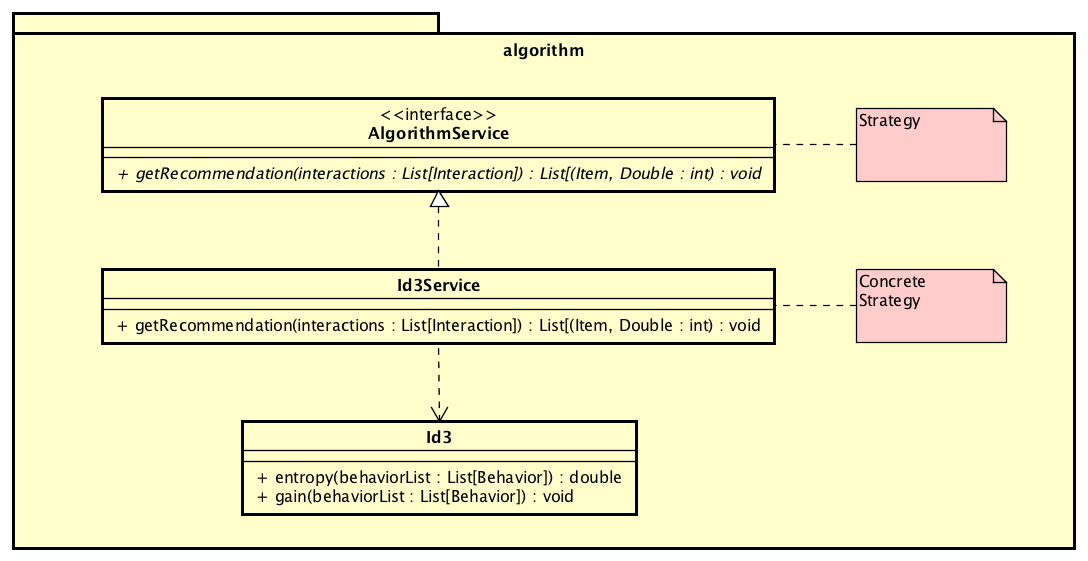
\includegraphics[width=0.9\linewidth]{immagini/strategyPattern}
\caption[Utilizzo del design pattern Strategy]{Utilizzo del design pattern Strategy}
\label{fig:strategyPattern}
\end{figure}

	\begin{itemize}
		\item \textbf{Descrizione:} \textit{pattern} comportamentale utilizzato per definire una famiglia di algoritmi, incapsularli e renderli intercambiabili;
		\item \textbf{Contesto d'utilizzo:} viene implementato nel \textit{package algorithm} dove dichiaro un'interfaccia che verrà invocata in base all'algoritmo prescelto.
	\end{itemize}
	\item \gls{singleton}
	\begin{figure}[h]
\centering
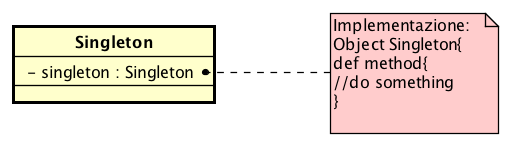
\includegraphics[width=0.9\linewidth]{immagini/singletonpattern}
\caption[Utilizzo del design pattern Singleton]{Utilizzo del design pattern Singleton}
\label{fig:singletonpattern}
\end{figure}

	\begin{itemize}
		\item \textbf{Descrizione:} \textit{pattern} \textit{creazionale} che ha la funzione di garantire un'unica istanza di una determinata classe;
		\item \textbf{Contesto d'utilizzo:} viene implementato nei \textit{package controller} e \textit{storage}.
	\end{itemize}
\end{itemize}

\newpage
\section{Progettazione di dettaglio}
\subsection{Interfaccia REST}
Di seguito sono elencate le risorse \gls{REST} associate al tipo di metodo che è possibile richiedere su di esse.
\begin{table}[h]
	\begin{tabular}{|p{0.5\textwidth}|p{0.4\textwidth}|}
		\toprule
		
		\textbf{Chiamata} & \textbf{Tipo risorsa}  \\
		\bottomrule
		\end{tabular}\\	
		\end{table}
		
		\begin{table}[h]
			\begin{tabular}{|p{0.5\textwidth}|p{0.4\textwidth}|}
				\toprule
				\textbf{/tres/ready} & \textbf{GET}  \\ \midrule
				\multicolumn{2}{|c|}{Controlla se l'algoritmo è in grado di fornire una raccomandazione.} \\
				\bottomrule
			\end{tabular}\\
				\par\bigskip
			
			\begin{tabular}{|p{0.5\textwidth}|p{0.4\textwidth}|}
				\toprule
				\textbf{/tres/behavior} & \textbf{POST}  \\ \midrule
				\multicolumn{2}{|c|}{Inserimento di un \textit{behavior} nel sistema.} \\
				\bottomrule
			\end{tabular}\\
				\par\bigskip
			
			\begin{tabular}{|p{0.5\textwidth}|p{0.4\textwidth}|}
				\toprule
				\textbf{/tres/recommendation} & \textbf{POST}  \\ \midrule
				\multicolumn{2}{|c|}{Calcola la raccomandazione da fornire ad un utente.} \\
				\bottomrule
			\end{tabular}\\
			\par\bigskip
		\end{table}
		
\subsection{Diagrammi di sequenza}
Si mostrano i diagrammi di sequenza di alcune chiamate \gls{REST} che effettua il sistema per meglio specificare il funzionamento.
\subsubsection*{Inserimento nuovo behavior}
Il diagramma sottostante illustra le operazioni necessarie all'inserimento di un nuovo \textit{behavior}. Da \textit{Bdrim} arriva una richiesta \textit{Http} che viene instradata alla classe \textit{BridgeController} mediante il file \textit{routes}. Il \textit{controller} invoca la funzione \textit{insertBehavior}, la quale valida il \gls{JSON} ricevuto e successivamente chiama il metodo \textit{save} della classe \textit{BehaviorDAO}.
\begin{figure}[h]
\centering
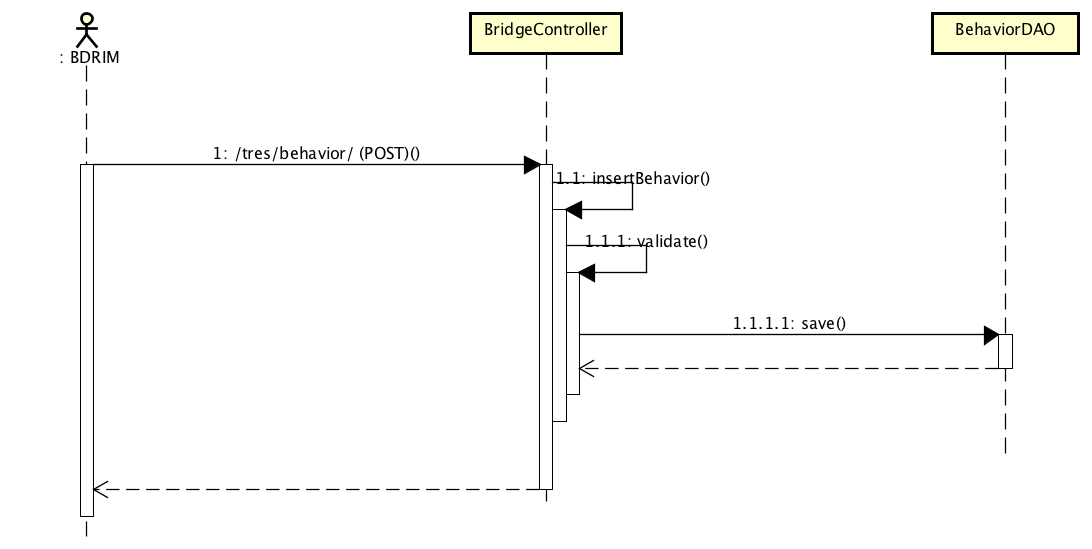
\includegraphics[width=0.9\linewidth]{immagini/sequenzaSalvabehavior}
\caption[Diagramma di sequenza: Inserimento nuovo behavior]{Diagramma di sequenza: Inserimento nuovo behavior}
\label{fig:sequenzaSalvabehavior}
\end{figure}

\newpage
\subsubsection*{Controllo dello stato}
Il diagramma sottostante illustra le operazioni necessarie per capire se l'algoritmo ha a disposizione abbastanza dati per fornire la raccomandazione. Da \textit{Bdrim} arriva una richiesta \textit{Http} che viene instradata alla classe \textit{BridgeController} mediante il file \textit{routes}. Il \textit{controller} invoca la funzione \textit{ready}. L'invocazione lancia a propria volta un'invocazione alla funzione \textit{ready} dell'interfaccia \textit{AlgorithmService}, il quale indica il successo o il fallimento del controllo.
\begin{figure}[h]
\centering
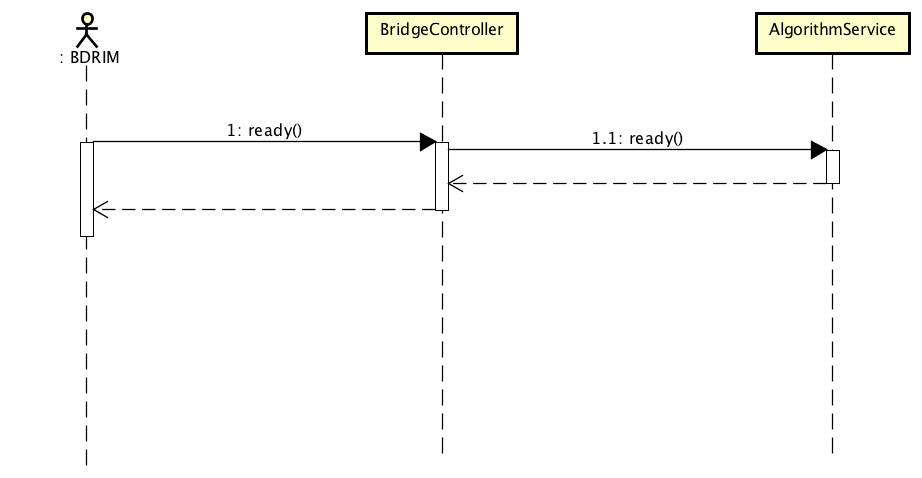
\includegraphics[width=0.9\linewidth]{immagini/sequenzaReady}
\caption[Diagramma di sequenza: Controllo dello stato]{Diagramma di sequenza: Controllo dello stato}
\label{fig:sequenzaReady}
\end{figure}


\section{Verifica e validazione}\label{metriche}
Ho adottato metriche specifiche e strumenti per l'analisi statica e dinamica al fine di perseguire gli obbiettivi di qualità, sia di processo che di prodotto. Per questo motivo è necessaria una costante verifica sulle attività svolte. Così facendo si permette di trovare possibili incongruenze e anomalie per poter intervenire in maniera tempestiva ed efficace.
Gli strumenti utilizzati sono i seguenti:
\begin{itemize}
	\item \textbf{Intellij IDEA\footnote{\url{https://www.jetbrains.com/idea/whatsnew/}}: }fornisce una soluzione automatica per trovare tutti gli errori di sintassi più comuni e la percentuale di documentazione del codice;
	\item \textbf{Codecov\footnote{\url{https://codecov.io/}}}: fornisce la percentuale che indica la porzione di codice sorgente coperta da test;
	\item \textbf{Spec2}\footnote{\url{https://www.playframework.com/documentation/2.3.x/ScalaTestingWithSpecs2}}: libreria del framework per lo sviluppo dei test sul codice.
\end{itemize}
Riporto di seguito un elenco delle metriche adottate:
\begin{itemize}
	\item \textbf{Attributi per classe:} un numero elevato di attributi all'interno della classe potrebbe indicare il bisogno di suddividere la classe in più sottoclassi. Ho stabilito, come range ottimale, i valori da 1 a 8;
	\item \textbf{Complessità ciclomatica:} misura direttamente il numero di cammini linearmente indipendenti attraverso il grafo di controllo di flusso. Ho stabilito, come range ottimale, i valori da 1 a 10;
	\item \textbf{Copertura dei commenti:} valore percentuale che indica se le varie classi e metodi sono corredati da commenti. Il valore minimo entro il quale ho deciso di rimanere è 80;
	\item \textbf{Copertura dei test:} valore percentuale che indica la porzione di codice sorgente coperta da test. Il valore minimo entro il quale ho deciso di rimanere è 70\%.
\end{itemize}
Considerando il tempo limitato a disposizione, mi sono concentrato sulla realizzazione di un numero sufficientemente alto di test di unità e integrazione.\\
Gli eventuali errori durante questa attività sono stati corretti. In seguito ho proseguito con i test di integrazione, verificando come la combinazione di più componenti funzionasse secondo le aspettative. Conclusi i test di integrazione, ho fatto un test all'intero sistema. Infine, negli ultimi giorni di stage, ho verificato che i requisiti obbligatori tracciati in fase di progettazione fossero tutti soddisfatti e in presenza del responsabile, ho fatto il collaudo del software, dimostrando il corretto funzionamento.\\

\subsection{Risultati test}
Di seguito riporto le tabelle in cui verranno descritti alcuni dei test di integrazione, di unità e di sistema effettuati per verificare il corretto funzionamento dell'applicativo e i risultati di tali test:
\newpage
\subsection*{Test di integrazione}
\begin{center}
	\begin{table}[h]
		\begin{tabular}{|l|p{0.7\textwidth}|l|c|}
			\toprule
			
			\textbf{Test} & \textbf{Descrizione} & Componente & \textbf{Stato} \\
			
			\midrule
			TI1 & Viene verificato che il sistema crei correttamente un albero di decisione & algorithm &  Success \\ \midrule
			TI2 & Viene verificato che il sistema aggiorni l'albero di decisione ogni 24 ore & algorithm & Success \\ \midrule
			TI3 & Viene verificata la corretta creazione del \textit{training set} & algorithm & Success \\ 
			\bottomrule
			
		\end{tabular}
		\caption{Tabella test di integrazione}
		
	\end{table}
	
\end{center}


\subsection*{Test di unità}
\begin{center}
	\begin{table}[h]
		\begin{tabular}{|l|p{0.7\textwidth}|l|}
			\toprule
			
			\textbf{Test} & \textbf{Descrizione} &  \textbf{Stato} \\
			
			\midrule
			TU1 & Viene verificato che il sistema salvi correttamente un comportamento all'interno del database & Success \\ \midrule 
			TU2 & Viene verificato il corretto caricamento di una lista di \textit{widgetTag} distinti   & Success \\ \midrule 
			TU3 & Viene verificato il corretto caricamento di una lista di \textit{item} distinti &  Success \\ \midrule
			TU4 & Viene verificato il corretto caricamento di una lista di \textit{behavior} con una  \textit{interaction} specifica & Success \\ \midrule
			TU5 & Viene verificato il corretto caricamento di una lista di \textit{behavior} con \textit{tag e action} specifici & Success \\ \midrule
			TU6 & Viene verificato il corretto caricamento di una lista di \textit{action} distinti & Success \\ \midrule
			TU7 & Viene verificato il corretto calcolo dell'entropia & Success \\ \midrule
			TU8 & Viene verificato il corretto calcolo del guadagno di informazione & Success \\ \midrule
			TU9 & Viene verificato che venga creata la raccomandazione corretta da fornire & Success \\ \midrule
			TU10 & Viene verificato il corretto calcolo delle probabilità & Success \\ 
			
			\bottomrule
			
		\end{tabular}
		\caption{Tabella test di unità}
		
	\end{table}
	
\end{center}

Prima di effettuare il collaudo, sono stati effettuati alcuni test di sistema, conclusi con successo, che hanno permesso di verificare il comportamento dinamico del sistema. 
\begin{itemize}
	\item \textbf{Inserimento dati}: viene verificato il corretto comportamento del sistema alla richiesta di inserimento dati;
	\item \textbf{Calcolo raccomandazioni:} viene verificato il calcolo della raccomandazione da fornire;
	\item \textbf{Calcolo probabilità:} viene verificato il calcolo delle probabilità associate ai vari \textit{item}.
\end{itemize}


\subsection*{Risultati delle misurazione del codice}
Sono di seguito riportati i risultati dei test di analisi statici effettuati sul codice:
\begin{itemize}
	\item \textbf{Complessità ciclomatica: }per il calcolo della complessità ciclomatica ho usato il \textit{tool SBT} \textit{"The interactice build tool"}\footnote{\url{http://www.scala-sbt.org/}}, il quale contiene all'interno un task denominato \textit{styleCheck} che segnala con un \textit{warning} se la complessità ciclomatica supera il valore 10. Non ho ricevuto alcun \textit{warning}.
	\item \textbf{Attributi per classe:}
	\begin{itemize}
		\item Valore medio: 2;
		\item Valore massimo 4;
	\end{itemize}
	\item \textbf{Copertura commenti:} il valore di copertura è del 100\%.
	\item \textbf{Copertura dei test:} il valore di copertura dei test è del 73\%.
\end{itemize}




